We  now discuss   syntax and semantics of  our specifications, and illustrate through examples.
 
\subsection{\textbf{Syntax, Semantics, Examples}}
% chopped below, for space
% Our specification language   supports scoped invariants,   method specifications, and {conjunctions}. 

\begin{definition} [Specifications Syntax]     We define the syntax  of  specifications, $S$:
\label{f:holistic-syntax}
\[
\begin{syntax}
\syntaxElement{S}{ }
		  {\syntaxline
				{\  \TwoStatesN {\overline {x:C}} {A}\  }
 				{\ \mprepostN{A}{p\ C}{m}{y}{C}{A} {A}\ } 
				{\ S\, \wedge \, S\ }
		 \endsyntaxline
 		}
\endSyntaxElement\ 
\syntaxElement{p}{ } 
 	 {\syntaxline
                                  {\    \prg{private} \ } 	
				 {\   \prg{public} \ } 	
		 \endsyntaxline
 		}
\endSyntaxElement 
\end{syntax}
\]


\end{definition}

In Def. \ref{f:holistic-wff}  later on we describe  well-formedness of $S$, but  we first discuss  semantics and some examples.
%To motivate this definition, we first define the semantics of these specifications, and show some examples.
%
\label{ssect:sem}
 % 
%The semantics of specifications uses  
%For the semantics we 
We use quadruples involving states: % rather than statements}:
${\satAssertQuadruple  \Mtwo  M     {A} \sigma {A'} {A''} }$ 
  says that   if $\sigma$ satisfies $A$, then any terminating scoped execution of its continuation (${\leadstoBoundedStarFin { \Mtwo\madd M}{\sigma}  {\sigma'} }$) will satisfy $A'$, and any intermediate reachable external state 
  (${\leadstoBoundedStar  {\Mtwo\madd M}{\sigma}  {\sigma''}}$) will satisfy the "mid-condition", $A''$. 
  
 
\begin{definition} \label{def:hoare:sem}
\label{def:shallow:spec:sat:state}
For modules $\Mtwo$, $M$, state $\sigma$, and assertions $A$, $A'$ and  $A''$, we define:
\begin{itemize}
\item
$ {\satAssertQuadruple  \Mtwo  M     {A} \sigma {A'} {A''} } \ \ \triangleq \ \ \forall \sigma',\sigma''.[
$  \\
$\strut \hspace{.2cm} M,  \sigma \models  {A}   
  \  \ \Longrightarrow \ \   [ \ \  {\leadstoBoundedStarFin { \Mtwo\madd M}{\sigma}  {\sigma'} }\ \ \Longrightarrow\ \   M,  \sigma' \models  {A'}  
 \ \ \ \  ] \ \ \ \wedge$\\ 
 $\strut   \   \hspace{2.5cm}  [ \ \   {\leadstoBoundedStar  {\Mtwo\madd M}{\sigma}  {\sigma''} }\ \  \ \Longrightarrow\   \   M,  \sigma'' \models  {(\extThis \rightarrow {\as \sigma {A''}} )}\ \ \  ] \ \ \ \ \ ]$ 
\end{itemize} 
\end{definition}

{\begin{example}
Consider ${\satAssertQuadruple  \Mtwo  M     {A_1} {\sigma_{4}} {A_2} {A_3} }$   
for Fig. \ref{fig:illusrPreserve}.
It says that  if  $\sigma_4$ satisfies $A_1$ 
then $\sigma_{23}$ will satisfy $A_2$, while $\sigma_6$-$\sigma_9$, $\sigma_{13}$-$\sigma_{17}$, $\sigma_{20}$-$\sigma_{21}$ will satisfy $A_3$.
It does not guarantee anything about $\sigma_{24}$ because $\notLeadstoBoundedStar {...} {\sigma_4} {\sigma_{24}}$.
Similarly, if $\sigma_8$ satisfies $A_1$ 
then $\sigma_{14}$ will satisfy $A_2$, and  $\sigma_9$ and $\sigma_{14}$  will satisfy $A_3$, while making no guarantees about  $\sigma_{15}$ onwards.
 \end{example}}

{Now to} % should have been "to the" but this way we avoid bad line break in 3 lines
 semantics of specifications:     $\satisfies{M}{\TwoStatesN {\overline {x:C}} {A}}$ 
says that if an external state $\sigma$ satisfies $A$, then all future external states reachable from $\sigma$—including nested  
 calls and returns but  {\emph{stopping} before}   returning from the active call in $\sigma$— also satisfy $A$. 
 And  $\satisfies{M} { \mprepostN {A_1}{p\ D}{m}{y}{D}{A_2} {A_3} }$ says that scoped execution of a call to $m$ from $D$   in  states satisfying $A_1$ leads to final states satisfying $A_2$ (if it terminates),
 and to intermediate external states satisfying $A_3$.

\begin{definition}  [Semantics of  Specifications]
We define $\satisfies{M}{{S}}$ by cases over $S$:  

\label{def:necessity-semantics}

\begin{enumerate}
 \item
\label{def:necessity-semantics-first}
 $\satisfies{M}{\TwoStatesN {\overline {x:C}} {A}} \ \  \ \triangleq   \ \ \ {\forall   \Mtwo,  \sigma.[\ {\satAssertQuadruple  \Mtwo  M    {\extThis \wedge \overline {x:C} \wedge A} \sigma {A} {A} }\ ].}$
  \item
   \label{def:necessity-semantics-second}
 $\satisfies{M} { \mprepostN {A_1}{p\ D}{m}{y}{D}{A_2} {A_3} }\  \ \ \   \triangleq  $ \\ %  \ \ \ \forall   \Mtwo,  \sigma, y_0,\overline y.[\ $    \\
$\strut \ \   \forall   \Mtwo,  \sigma, y_0,\overline y.[\ 
% $\\ $\strut  \ \ \   \ \ \ \ \ \ \ \ \   \  \ \ \
 \ \sigma.\prg{cont}\txteq {u:=y_0.m(y_1,..y_n)} \ \ \Longrightarrow \ \ $\\
$\strut  \ \ \   \ \ \ \ \ \ \ \ \   \ \ \  \ \ 
\ \ \ \ \ \ \ \ \ {\satAssertQuadruple  { \Mtwo} {M} { y_0\!:\!D, \overline {y\!:\!D}   \wedge   A[y_0/\prg{this}]}  {\ \sigma\ }   {A_2[u/res,y_0/\prg{this}] }{A_3 } } \  \ \  ]  $   
%$\strut  \ \ \   \ \ \ \ \ \ \ \ \   \  \mbox{where}$\\
%$\strut  \ \ \   \ \ \ \ \ \ \ \ \   \   A_1' \triangleq   y_0:D,{\overline {y:D}}   \wedge   A[y_0/\prg{this}],\  \  A_2' \triangleq A_2[u/res,y_0/\prg{this}],\ \ A_3' \triangleq A_3  \  ]$  
 \item
 $\satisfies{M}{S\, \wedge\, S'}$\ \ \  \ \ \  $\triangleq$  \  \ \  \   $\satisfies{M}{S}\ \wedge \ \satisfies{M}{S'}$
\end{enumerate}
\end{definition}

Fig. \ref{fig:illusrPreserve} in  \S \ref{sect:approach:scoped}  illustrated  the meaning of ${\TwoStatesN {\overline {x:C}} {A}}$. 
Moreover, $M_{good} \models S_2 \wedge S_3 \wedge S_4$, and  $M_{fine} \models S_2 \wedge S_3 \wedge S_4$,
 while $M_{bad} \not\models S_2$.
We continue with some examples -- more in % can be found in 
\A ~\ref{app:spec}.

{
 \begin{example}[Scoped Invariants and Method Specs]
 \label{example:twostate}
 \label{example:mprepostl}
  % 
 $S_5$  says % shorter than guarantees  
  that   non-null keys are immutable:
 \\
 \begin{tabular}{lcll}
$\strut \ \ \ \ \ \ \ \ S_5$ & $\triangleq$   & ${\TwoStatesN {\prg{a}:\prg{Account}.\prg{k}:\prg{Key}}  {\prg{null}\neq \prg{k}=\prg{a.\password}}} $  \end{tabular}
\\
% \end{example} 
% }
%
%
% 
% \begin{example}[Method Specifications]
% \label{example:mprepostl}
 %A specification for method \prg{buy} appeared in \S\ref{sec:howThird}. 
%(Method Specifications) Here,  
$S_9$    guarantees that \prg{set} preserves the protectedness of any account, and any key.  \\
%   \small   {
%  {\sprepost
%		{\strut \ \ \ \ \ \ \ \ \ S_6} 
%		{   \protectedFrom{\prg{this}.\prg{\myAccount}.\prg{key}} {\prg{buyer}} \wedge \prg{this}.\prg{\myAccount}.\prg{\balance}=b
%		 }
%		{\prg{public Shop}} {\prg{buy}} {\prg{buyer}:\prg{external}, \prg{anItem}:\prg{Item} }
%		{ 
%		  \protectedFrom{\prg{this}.\prg{\myAccount}.\prg{key}} {\prg{buyer}} \wedge \prg{this}.\prg{\myAccount}.\prg{\balance}\geq b
%		 }}
%  }
%  \\
%  \small {
   {\sprepost
		{\strut \ \ \ \ \ \ \ \ \ S_9} 
		{  a:\prg{Account}, a':\prg{Account}\wedge  \inside{a}\wedge  \inside{a'.\prg{key}} }
		{\prg{public Account}} {\prg{set}} {\prg{key'}:\prg{Key}}
		{   \inside{a}\wedge  \inside{a'.\prg{key}}  }
		{   \inside{a}\wedge  \inside{a'.\prg{key}} }
}

\noindent
Note that  $a$, $a'$ are disjoint from \prg{this} and the formal parameters of \prg{set}. 
In that sense, $a$ and $a'$ are universally quantified; a call of \prg{set} will preserve protectedness for \emph{ all} accounts and their keys. 

\end{example}

\subsection{\textbf{Well-formedness}} We now define what it means for a specification to be well-formed:

\begin{definition}% [Specifications Well-formed]    
 {\emph{Well-formedness}} of specifications,  $\vdash S$,  is   defined by cases on $S$:
\label{f:holistic-wff}

\begin{itemize}
\item
  $\strut \  \vdash {\TwoStatesN {\overline {x:C}} {A}} \ \ \ \triangleq\  \ \ \fv(A)\subseteq\{  \overline x \}\,\wedge\, {M \vdash \encaps {{\overline {x: C}} \wedge A}} $.
    \item
 $\strut \ \vdash {\mprepostN{\overline{x:C'} \wedge A}{p\ C}{m}{y}{C}{A'} {A''}}\ \ \ \triangleq$\\
$\strut \hspace{0.7cm}  [ \ \ {\small{   {\prg{res},\prg{this}\!\notin\! \overline{x}, \overline{y}}\ \wedge\  {\fv(A)\!\subseteq\! \overline x, \overline y, \prg{this}}\     \wedge\    \fv(A')\!\subseteq \! \overline{x}, \overline{y}, \prg{this}, \prg{res}\   \wedge\   \fv(A'')\!\subseteq\!  {\overline{x}} }} $\\
    $\strut \hspace{0.7cm} \ \ \  \wedge\  \Pos {A } \, \ \wedge \ \,  \Pos {A'} \, \ \wedge \  \,  M \vdash \encaps  {\overline {x: C'} \wedge A''}\ \ \  ]$ 
%  \item
% SAME AS ABOVE, not small, and in 3 lines
% $\strut \ \vdash {\mprepostN{\overline{x:C'} \wedge A}{p\ C}{m}{y}{C}{A'} {A''}}\ \ \ \triangleq$\\
%  $\strut \hspace{1cm} [ \ \  {\prg{res},\prg{this}\notin \overline{x}, \overline{y}} \ \ \wedge$\\
% $\strut \hspace{1cm} \ \ \ \  {\fv(A)\subseteq \overline x, \overline y, \prg{this}}\  \,  \wedge\ \,  \fv(A')\subseteq    \overline{x}, \overline{y}, \prg{this}, \prg{res}\  \, \wedge\ \,  \fv(A'')\subseteq  {\overline{x}}\ \  \wedge $\\
%    $\strut \hspace{1cm} \ \ \ \   \Pos {A \wedge A' \wedge A''} \, \ \wedge \  \,  M \vdash \encaps  {\overline {x: C'} \wedge A''}\ \ \  ]$ 
  \item  $\strut \   \vdash S\, \wedge \, S' \ \ \triangleq \ \  \vdash S\, \ \wedge\,  \ \vdash S'  $.  
\end{itemize}

\end{definition}

Def \ref{f:holistic-wff}'s  requirements about  free variables are relatively straightforward -- more  in. \S \ref{wff:spec:free:more}.

%Def \ref{f:holistic-wff}'s  requirements about encapsulation are more interesting:
Def \ref{f:holistic-wff}'s  requirements about encapsulation are motivated by  Def.   \ref{def:necessity-semantics}. If  $\overline {x:C}\wedge A$ in the scoped invariant  were not encapsulated,  then it could be invalidated by some external code, and it would be impossible to ever satisfy Def.   \ref{def:necessity-semantics}(\ref{def:necessity-semantics-first}). % requirement that $A$ is preserved during scoped external execution.
Similarly, if a method specification's mid-condition, $A''$, could be invalidated by some external code, then it would be impossible to ever satisfy Def.   \ref{def:necessity-semantics}(\ref{def:necessity-semantics-second}). % requirement that $A''$ holds in intermediate external states.


Def \ref{f:holistic-wff}'s  requirements about stability are motivated by our Hoare logic rule for internal calls,   {\sc{[Call\_Int]}}, Fig \ref{f:internal:calls}. The requirement    $\Pos {A}$ for the method's precondition, gives that $A$ is preserved when an internal frame is pushed, \cf Lemma \ref{l:preserve:asrt}.
The requirement     $\Pos {A'}$ for the method's postcondition gives,  in the context of \strong satisfaction,  that $A'$ is preserved when an internal frame is popped, \cf Lemma \ref{l:calls:return:deep}. This is crucial for soundness of  {\sc{[Call\_Int]}}.

  %precondition's free variables all appear in the formal parameters or 
%{\emph{Well-formedness}},  $\vdash S$,  is   defined by cases on $S$:\\
%  $\strut \ \  \vdash {\TwoStatesN {\overline {x:C}} {A}} \ \ \ \triangleq\  \ \ \fv(A)\subseteq\{  \overline x \}\,\wedge\, {M \vdash \encaps {{\overline {x: C}} \wedge A}} $;\\
% $\strut \ \  \vdash {\mprepostN{A}{p\ C}{m}{y}{C}{A'} {A''}}\ \ \ \triangleq\  \ \  \exists \overline x, \overline {C'}.[ $\\
%  $\strut \hspace{1cm}  {\prg{res}\notin \overline{x}, \overline{y}}\,  \wedge\,  \ {\fv(A_0)\subseteq \overline{x},\overline y, \prg{this}}\   \wedge \fv(A')\subseteq  \fv(A),\prg{res}\   \wedge\  \fv(A'')\subseteq  {\overline{x}} $\\
%  $\strut \hspace{1cm}\wedge\  \Pos A\, \wedge\, \Pos {A'}\, \wedge \,\Pos {A''}\, \wedge  \,  M \vdash \encaps  {\overline {x: C'} \wedge A''}\ \ \  ]$ \\
%  $\strut \ \   \vdash S\, \wedge \, S' \ \ \triangleq \ \  \vdash S\, \wedge\, \vdash S'  $.  



\subsection{\textbf{Discussion}}  

\paragraphSD{Difference with Object and History Invariants}  Our scoped invariants are similar to, but different from, history invariants  and object invariants, but
neither of these provide what we need. 
We compare through an example:

\vspace{-.35cm}
 
\noindent
\begin{flushleft}
\begin{tabular}{@{}lr@{}}
  \begin{minipage}{.85\textwidth}
Consider $\sigma_a$ making a call  transitioning to $\sigma_b$,    execution of $\sigma_b$'s continuation   eventually resulting in $\sigma_c$, and $\sigma_c$ returning  to $\sigma_d$. 
Suppose all four states are external, and the module guarantees $\TwoStatesN {\overline{x:Object}} {A}$, and $\sigma_a \not\models A$, but $\sigma_b \models A$. 
Scoped invariants %require   
ensure  $\sigma_c \models A$, but allow   $\sigma_d \not\models A$.\end{minipage}
& 
\begin{minipage}{.18\textwidth}
\resizebox{2cm}{!}{
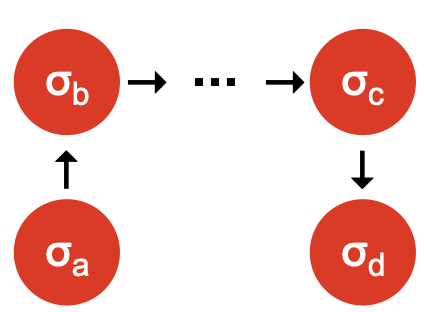
\includegraphics[width=\linewidth]{diagrams/compare.png}
} 
\end{minipage}
\end{tabular}
\end{flushleft}


{\emph{History  invariants}} \cite{liskov94behavioral,usinghistory,Cohen10}, instead, consider {all  future states including any method returns}, and therefore {would  require that   $\sigma_d \models A$. Thus, they are,}  for our purposes,  both
 \emph{unenforceable} and overly \emph{restrictive}.\ \  \emph{Unenforceable}: \ Take $A \txteq \inside{\prg{acc.key}}$,  assume  in $\sigma_a$ a path to an external object which has access to $\prg{acc.key}$, assume that path is unknown in $\sigma_b$: then, the transition from $\sigma_b$ to $\sigma_c$ cannot eliminate that path—hence, $\sigma_d \not\models \inside{\prg{acc.key}}$.\ \  \emph{Restrictive}:\ Take $A \txteq \inside{\prg{acc.key}}\wedge a.\prg{blnce}\geq b$; then,  requiring  $A$   to hold in all states from $\sigma_a$ until termination would prevent all future withdrawals from $a$, rendering the account useless.

{\emph{Object}} invariants  \cite{Meyer92,MeyerDBC92,BarDelFahLeiSch04,objInvars,MuellerPoetzsch-HeffterLeavens06}, on the other hand, expect %require -- too many require in the para
invariants to hold in all (visible) states,
here would require,  \eg that $\sigma_a \models A$. Thus, they  are %equally 
\emph{inapplicable} for us: They would require, \eg, that for all % objects 
 $\prg{acc}$, in all (visible) states, $\inside{\prg{acc.key}}$, and thus prevent \emph{any} withdrawals from \emph{any} account in \emph{any} state.
 
 

\paragraphSD{Difference between Postconditions and Invariants}
% The interested reader might have noticed that 
In all  method specification examples so far, the post-condition and   mid-condition were identical.
However, this need not be so. 
Assume a method \prg{tempLeak} defined in \prg{Account}, with an external argument \prg{extArg}, and  method body:
\\
{\small{$\strut \hspace{1cm} \prg{extArg.m(this.key); this.key:=new Key}$}}
\\
Then, the assertion   $ \inside{\prg{this.key}}$  is  invalidated by the external call \prg{extArg.m(this.key)}, but is  established by \prg{this.key:=new Key}.
Therefore, $ \inside{\prg{this.key}}$  is a valid post-condition but not a valid   mid-condition.
The specification of \prg{tempLeak} could be\\
{\small{$
{\sprepost
		{\strut \ \ \ \ \ \ \ \ \ S_{\prg{tempLeak}}} 
		{  \ \prg{true}\  }
		{\prg{public Account}} {\prg{tempLeak}} {\prg{extArg}:\prg{external}}
		{  \  \inside{\prg{this.key} }\  }
		{  \  \prg{true}\  }
}
$}}

 
 
\footnoteSD{First bullet: This means that we require all objects to satisfy even if not locally relevant. Second Bullet: notice that we are asking for globally relevant objects}  
\footnoteSD{{TODO: Make an example that demonstrates the difference if in the second bullet we had asked for locally relevant objects ${\overline o}$.}}
\footnoteSD{TODO: explain why we did not require the stronger $\leadstoFin{M_{ext}\!\circ \!M}{\sigma}{\sigma'}$ rather than $\leadstoBoundedStar {M_{ext}\!\circ \!M}{\sigma}  {\sigma'}$.}

\newcommand{\paragraphSDD}[1]{\vspace{.02cm}{\textit{#1}}}
 
\subsection{Expressiveness} 

We argue the expresseness of our approach  through a sequence of capability patterns studied in related approaches from the literature  
 \cite{OOPSLA22,dd,VerX,irisWasm23} written in our specification language.
These approaches %in  \cite{OOPSLA22,dd,VerX,irisWasm23}  
 are based on temporal logics \cite{VerX,OOPSLA22}, or on extensions of Coq/Iris \cite{dd,irisWasm23}, and
none offer a Hoare logic    for external calls.
%Other approaches in the literature are either unable to handle external method calls \cite{OOPSLA22}, or use  bespoke proofs \cite{dd,irisWasm23}, or model checking \cite{VerX}.
%Their specification languages are based on temporal logics \cite{VerX,OOPSLA22}, or on extensions of Coq and Iris \cite{dd,IrisWasm23}.
More in  \S \ref{app:expressivity}. 
% we argue our approach is able to prove comparable specifications to those proposed in  \cite{OOPSLA22,dd,VerX,irisWasm23}, in the presence of external method calls, using a Hoare logic.=≠≠≠q±±≠≠≠qq≠q≠≠www≠≠
We   summarize here.

 %% We continue the comparison of expresiveness between \emph{Chainmail} and \Nec, by 
 %% considering the examples studied in \cite{FASE}.
 
%\begin{example}[ERC20]

\paragraphSDD{DOM} % is the motivating example  in \cite{dd}:
Access to any DOM node
gives read/write  permissions to  all its \prg{parent} and \prg{children} nodes. 
These permissions are attenuated   through a \prg{Proxy} class, %which has a field \prg{node} pointing to a \prg{Node}, and a field \prg{height}, 
 which restricts the range of \prg{Node}s which may be modified through the use of the particular \prg{Proxy}. 
We  express such  attenuation   through two scoped invariants.
% The corresponding specification in \ref{OOPSLA22} is comparable, but not able to prove external calls. % not specific as to the frame from which any modification originated.

\paragraphSDD{DAO} %Decentralized Autonomous Organization\
 ~\cite{Dao}  is a well-known Ethereum contract   which was exploited with a re-entrancy bug in 2016, 
and lost \$50M. 
Our two state invariants  would have secured %the DAO 
 against that bug. % such a  bug. 
But note  that  they are about precluded effects, and 
%. They are, essentially, simple object invariants and 
thus expressible % could have been expressed 
 with techniques proposed in the 90's \cite{MeyerDBC92}.
% \cite{OOPSLA22}  gives one  further specification, which says  that any reduction of funds can only be caused through a call to a specific method -- such specifications are beoind our scope.
 
 \paragraphSDD{ERC20} is a widely used % token 
 standard describing  basic functionality of Ethereum-based token 
contracts. 
The Solidity security model is not based on access to  capabilities but on who the caller  is. 
We  adapted our approach correspondingly, and 
express 1) that  the owner of an account is always authorized on that account,  2) any execution which does not contain calls from a participant  authorized on some account will not affect the balance nor  who is authorized on  that account. 
% The specifications from \cite{OOPSLA22} are more API-specific, in that they pinpoint which method calls caused an effect, and less specific in that they do not pinpoint the frame from which the effect occurred. 

\paragraphSDD{Stack} is a Wasm module exporting separate functions to read or modify its contents \cite{irisWasm23}. We specify that in the absence of external access to the latter capability, the contents will not change.  


 

%% KEEP ALL BELOW, but currently not needed 
%\subsection{\SpecLang Entailments}
%
%{We define entailment of specifications wrt a module in the expected way.} %The usual definition of entailment applies to our specifications as well}
%
%\begin{definition}[Satisfaction of Assertions by a module] 
%\label{def:assertion-inference-semantics}
%We define satisfaction of an assertion $A$ by a  module $M$ as:
%\begin{itemize}
%\item
%{
%$M \models A$   \ \ \ iff \ \ \  $\forall \overline{M}. \forall \sigma
%[\ \    \arising{\sigma}{M\madd\overline{M}}\   \  \wedge\ \  \satisfiesA {M}   {\sigma} {\external{\prg{this}}} 
%\   \ \Longrightarrow \ \ \satisfiesA{M}{\sigma}{A}\ \ ]$
%}\footnote{Not sure about the need for external and arising.}
%\end{itemize}
%\end{definition}
%
%%TODO: Here we will say that assertions are classical, as proven in FASE
%
%\begin{definition}[Stronger Specifications] 
%\label{def:specification-implication-semantics}
%Specification $S$ is stronger than another specification $S'$  in the context of a  module: 
% \begin{itemize}[itemsep=5pt]
%\item 
%$\stronger M  S  {S'}$   \ \ \ iff \ \ \  $M\models S$ implies $M \models S'$
%\item
%$\strongerEq M  S  {S'}$   \ \ \ iff \ \ \ $\stronger M  S  {S'}$  \ and \  $\stronger M   {S'} S$    
%\end{itemize}
%\end{definition}
%
%\noindent
%{Interestingly, entailment can deduce some method specifications out of two-state invariants.}
%
%{
% \begin{example}
% \label{example:entail}
% Any module $M$ whose code does not call  method \prg{buy} gives   $\stronger M {S_2 \wedge S_S4} {S_9}$
%\end{example}
%
%
%% Remember $S_1$, ... $S_4$ as defined in Sect. \ref{s:bankSpecEx}, and consider the specifications $S_6$ and $S_7$ from Example \ref{example:mprepostl}.
%% Then, for any module $M$ %which has a public method \prg{set}, 
%% we have that
%\begin{example}
% \label{example:entail}
%For any module $M$,  we have  $\strongerEq M {S_2 \wedge S_4} {S_2 \wedge S_{4a}}$, where $S_{4a}$ defined as 
%\\
%\begin{tabular}{lcll}
%  $S_{4a}$   & $\triangleq$   &  
% $ \TwoStatesQ{\prg{a}:\prg{Account},\prg{b}:\prg{int}}  {\inside{\prg{a.\password}} \wedge \prg{a.\balance}\geq\prg{b}} 
% {\inside{\prg{a.password}} \wedge \prg{a.\balance}\geq\prg{b}} $
% \end{tabular}
%\ \end{example}
%}
% 
%%Some properties of $M \models \_  \subseteq \_ $ are given below:
%%
%%\begin{lemma}
%%For assertions $A$, $A'$, variables $\overline y$, and $\overline x$, specifications $S$, $S'$, $S''$, and module $M$:
%%\begin{itemize} [topsep=6pt,itemsep=5pt,parsep=0pt,partopsep=0pt]
%%%\item
%%% $\stronger M {\OneStateQ {\overline {x:C}}  {A}}  {\TwoStatesQ {\overline {x:C}} {A}{A}} $ 
%%%    \item
%%%  $\strongerEq  M  {\OneStateQ    {y:\prg{Object}}   {\forall \overline {x:C}[ A ] } } 
%%%    {\OneStateQ {\overline {x:C}}  {A}} $.
%%\item
%%$\strongerEq M    {\TwoStatesQ {\overline {x:C}} {A}{A'}}    {\TwoStatesQ {\overline {y:C}} {A[y/x]}{A'[y/x]}}$
%%\item
%%$  M  \models    \overline {x:C} \wedge A_1'  \rightarrow A_1$ \ \ \  and \ \ \
%%$  M  \models  \overline {x:C} \wedge A_2'  \rightarrow A_2$  \ \ \ \ 
%%implies\\
%% $\strut \hspace{5cm} \stronger M  {\TwoStatesQ {\overline {x:C}} {A_1}{A_2}}     {\TwoStatesQ {\overline {x:C}} {A_1'}{A_2'}}$
%%
%%\item
%%$\stronger M  S {S''}$ and $\stronger M {S''} {S'}$\ \  \ implies\  \ \ $\stronger M S  {S'}$.
%%
%%\end{itemize}
%%
%%\end{lemma}


%%%%%%%%%%%%%%%%%%%%%%%%%%%%%%%%%%%%%%%%%%%%%%%%%%%%%%%%%%%%%%%%%%%%%%


